\section{Unit Manager} \label{sec:unitmanager}

The Unit Manager is an INTENS component that handles the automatic
scaling of values in the user interface.

\begin{figure}[h]\label{fig:unitmanager}
  \begin{center}
    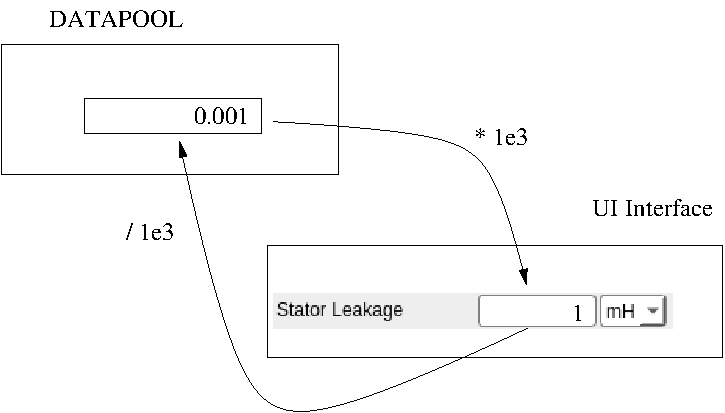
\includegraphics[width=0.7\linewidth]{xfig/unitmanager}
  \end{center}
  \caption{Automatic Scaling}
\end{figure}

The units can be configured. In INTENS included is a set of
standard units. For example
\begin{lstlisting}[language=json, escapeinside={(*}{*)}]
[...,
 {"name": "H", "factor": 1.0,
 "derived": [
     {"name": "mH", "factor": 1e3},
     {"name": "(*$\mu$*)H", "factor": 1e6}
 ]},
 ...
]
\end{lstlisting}
This produces a set (combobox) with 3 entries: H, mh, $\mu$H
and H as the base unit (ie. the unit of the values in the datapool).

If a single value ``mH'' is preferred the following configuration
can be written to the file

\verb+etc/application_unit.json+:
\begin{lstlisting}[language=json]
{"name": "H", "factor": 1.0, "use_set": 0,
"derived": [
    {"name": "mH", "factor": 1e3}
]}
\end{lstlisting}
The value ``\verb+use_set+'' controls the content of the set.
Only units with ``\verb+use_set+'' value 1 (which is default)
are included.
